\documentclass[t]{beamer}
\usetheme[deutsch]{KIT}
\setbeamercovered{transparent}
\setbeamertemplate{navigation symbols}{}

\KITfoot{Tutoriumsmaterial von Joachim Priesner, Sebastian Ullrich und Max Wagner \hspace{2.5cm} Basierend auf den Folien von Simon Stroh und Moritz v. Looz}
\usepackage[utf8]{inputenc}
\usepackage{amsmath}
\usepackage{ifthen}
\usepackage{amssymb}
\usepackage{tikz}
\usepackage{ngerman}
\usetikzlibrary{automata}
\usenavigationsymbols


\title{Theoretische Grundlagen der Informatik}
\subtitle{Tutorium}
\author{Moritz von Looz, Simon Stroh}

\institute[ITI]{Institut für Theoretische Informatik}

\TitleImage[height=\titleimageht]{images/tmaschine.png}

\newcommand{\N}{\ensuremath{\mathbb{N}}}
\newcommand{\M}{\ensuremath{\mathcal{M}}}
\newcommand{\classP}{\ensuremath{\mathcal{P}}}
\newcommand{\classNP}{\ensuremath{\mathcal{NP}}}
\newcommand{\co}{\ensuremath{\mathsf{co\text{-}}}}
\newcommand{\pot}{\ensuremath{\mathcal{P}}}
\newcommand{\abs}[1]{\ensuremath{\left\vert #1 \right\vert}}
\newcommand{\menge}[2]{\ensuremath{\left\lbrace #1 \,\middle\vert\, #2 \right\rbrace}}
\newcommand{\ducttape}[1]{\vspace{#1}}
\newcommand{\neglit}[1]{\overline{#1\vphantom{x^a}}}
\newcommand{\recipe}{\raisebox{-.3cm}{
\includegraphics[scale=.15]{images/chefs-cap.png}}\hspace{0.2cm}}

\newcommand{\invincible}{\setbeamercovered{invisible}} %  "Yesss! I am invincible!!" (Boris Grishenko)
\newcommand{\vincible}{\setbeamercovered{transparent}}

% \@ifundefined{tikzset}{}{\tikzset{initial text=}} % Text "start" bei Startknoten unterdrücken
\tikzstyle{every node}=[thick]
\tikzstyle{every line}=[thick]

\newcommand{\tutnr}[1]{
  \subtitle{Tutorium #1}
	\begin{frame}
		\maketitle
	\end{frame}
}

\newcommand{\uebnr}[1]{
  \subtitle{Anmerkungen zum #1. Übungsblatt}
	\begin{frame}
		\maketitle
	\end{frame}
}

\begin{document}

\tutnr{7}

\section{Wiederholung}
\subsection{}

\begin{frame}
\frametitle{Allgemeines zu $\classNP$-Vollständigkeitsbeweisen}
In der Regel ist es schwer zu zeigen, dass ein Problem $\mathcal{NP}$-schwer ist, aber leicht zu zeigen, dass ein Problem in $\mathcal{NP}$ liegt.\\[8pt]
Da man üblicherweise ein $\mathcal{NP}$-vollständiges Problem als Voraussetzung für die Reduktion benötigt (Ausnahme: Satz von Cook), lohnt es sich einige kennen zu lernen.
\end{frame}

\section{SAT \& Co.}
\subsection{}

\begin{frame}
\frametitle{SAT}
\begin{block}{Problem}
\textbf{Gegeben:}
\begin{itemize}
 \item Menge $U$ von Variablen
 \item Menge $C$ von Klauseln (Disjunktionen) über $U$
\end{itemize}
\textbf{Frage:} Existiert eine (alle Klauseln) erfüllende Wahrheitsbelegung von $C$?
\end{block}
\begin{itemize}
\item \emph{Das} Standardproblem.
\item Es gibt viele hochoptimierte "`SAT-Solver"'. Steht man in der Praxis vor einem $\mathcal{NP}$-Problem, kann es sich anbieten, die Transformation auf $SAT$ durchzuführen.
\end{itemize}
\end{frame}
\begin{frame}
\frametitle{3SAT}
\begin{block}{Problem}
\textbf{Gegeben:}
\begin{itemize}
 \item Menge $U$ von Variablen
 \item Menge $C$ von Klauseln über $U$, jede Klausel enthält genau \emph{drei} Literale
\end{itemize}
\textbf{Frage:} Existiert eine erfüllende Wahrheitsbelegung von $C$?
\end{block}
\begin{itemize}
\item Bietet sich bei Reduktion eher an als $SAT$, da übersichtlicher
\end{itemize}
\end{frame}
\begin{frame}
\frametitle{MAX2SAT}
\begin{block}{Problem}
\textbf{Gegeben:}
\begin{itemize}
 \item Menge $U$ von Variablen
 \item Menge $C$ von Klauseln über $U$, wobei jede Klausel genau zwei Literale enthält
 \item Zahl $K \in \mathbb{N}$
\end{itemize}
\textbf{Frage:} Existiert eine Wahrheitsbelegung, die mindestens $K$ Klauseln erfüllt?
\end{block}

\begin{itemize}
	\item $MAX2SAT$ ist $\classNP$-vollständig, aber $2SAT$ ist in $\classP$.
\end{itemize}
\end{frame}

\begin{frame}
	\frametitle{Aufgabe}
	
	Haben die folgenden SAT-Instanzen eine Lösung? Gib eine erfüllende Wahrheitsbelegung an oder zeige, dass keine existieren kann.
\begin{enumerate}
 \item $\{a \vee b \vee \neglit{c}, b \vee c, \neglit{a} \vee \neglit{b} \vee \neglit{c}\}$
 \item $\{\neglit{a} \vee b, \neglit{b} \vee  a, a \vee b \vee \neglit{c}, \neglit{a} \vee c, \neglit{a} \vee \neglit{b} \vee \neglit{c}, \neglit{c} \vee \neglit{b}, a \vee b \vee c\}$
\end{enumerate}
\end{frame}

\section{Komplementsprachen}
\subsection{}

\begin{frame}
\frametitle{Komplementsprachen}
\begin{block}{Definition}
Zu einer Sprache $L \subseteq \Sigma^*$ definieren wir $\co L$ als das Komplement der Sprache, also
$\co L := \Sigma^*\setminus L$.
\end{block}
Für eine Klasse von Sprachen wie $\classP$ definieren wir die "`co"'-Klasse (wie z.B. $\co\classP$) als Menge der Komplemente (und nicht etwa als Komplement der Klasse -- warum?).\\[8pt]
\pause
Beispiele: \co 3SAT: Die aussagenlogischen Formeln mit 3 Variablen pro Klausel, die nicht erfüllbar sind.\\[8pt]

\pause
Aufgabe: Beschreibe \co SUBSET SUM\\[8pt]

\pause
Aufgabe: Gelten folgende Behauptungen?
\begin{itemize}
    \item $\classP = \co\classP$ ?
    \item $\classNP = \co\classNP$ ?
    \invincible \pause
    \item $\classNP \neq \co\classNP \Rightarrow \classP \neq \classNP$ ?
    \vincible
\end{itemize}
\end{frame}

\section{Graphenprobleme}
\subsection{}

\begin{frame}
\frametitle{Aufgabe}
Betrachte das Problem INDEPENDENT SET (IS):

\begin{itemize}
 \item Gegeben: Graph $G=(V, E)$, Parameter $K \leq |V|$
 \item Frage: Gibt es eine unabhängige Menge der Größe $K$ in $G$, d.h.~ eine Menge $V' \subseteq V$, mit $|V'| \geq K$, sodass $\{v, w\} \notin E$ für alle $v, w \in V'$? 
\end{itemize}

\only<1> {

Finde in folgendem Graphen $G_1 = (V_1, E_1)$ eine unabhängige Menge maximaler Größe:

\begin{center}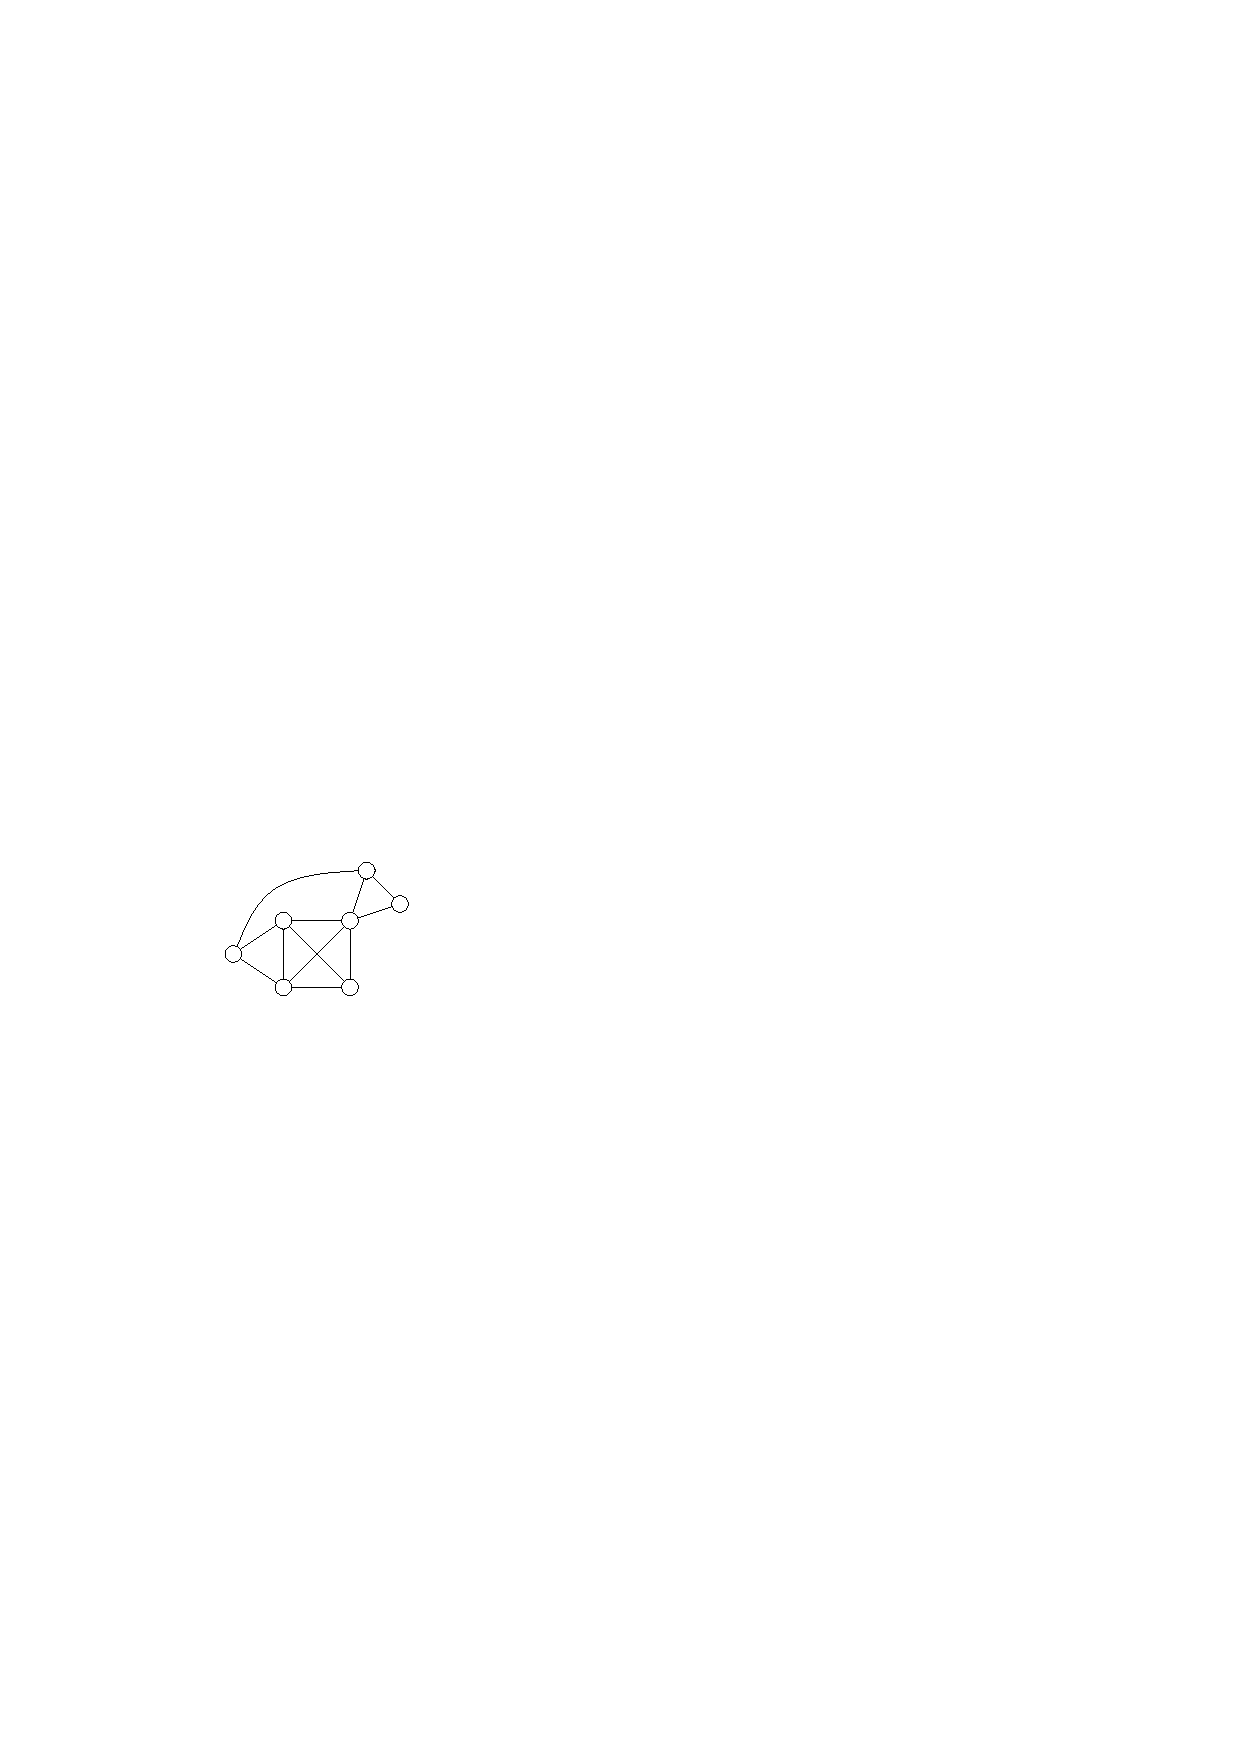
\includegraphics[scale=1.5]{images/tut7-graph}\end{center}

}

\only<2> {
	Formuliere das komplementäre Problem co-INDEPENDENT SET.
}

\only<3> {
	Zeichne $\overline{G_1}=(V_1, \overline{E_1})$, wobei $\overline{E_1}=\{\{v, w\} \mid v, w \in V_1, \{v,w\} \notin E_1\}$.
	
        Bestimme eine Clique maximaler Größe in $\overline{G_1}$.
        
        Was fällt dabei auf?
}

\only<4> {

Beweise die $\mathcal{NP}$-Vollständigkeit von IS. Gehe dabei wie folgt vor:
\begin{enumerate}
 \item Zeige: IS $\in \mathcal{NP}$.
 \item Zeige: $V'$ Clique in $G \Longleftrightarrow$ $V'$ unabhängige Menge in $\overline{G}=(V, \overline{E})$, wobei $\overline{E}= \menge{\{v, w\}}{v, w \in V, \{v, w\} \notin E}$
 \item Zeige, dass IS $\mathcal{NP}$-schwer ist.
\end{enumerate}

\raggedleft{\vspace{-.5cm} 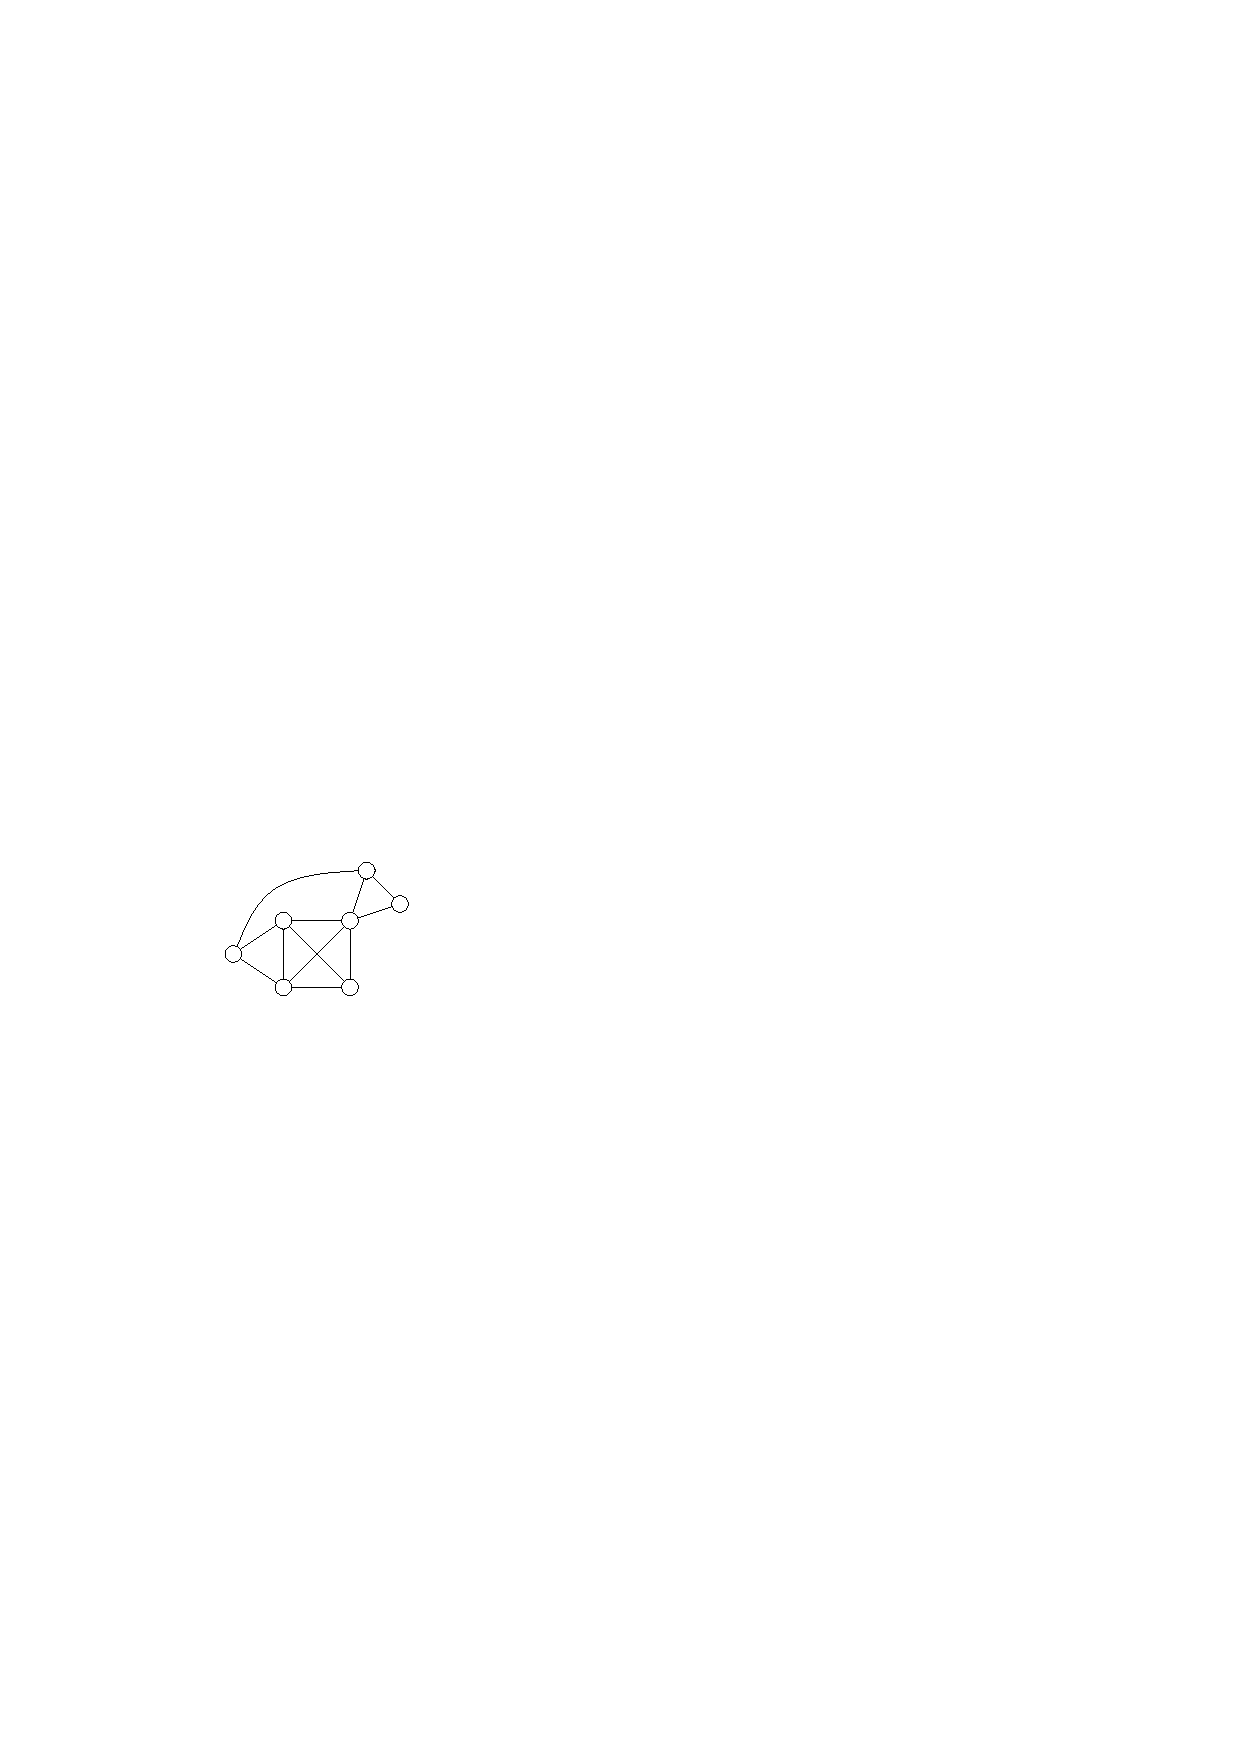
\includegraphics[scale=1]{images/tut7-graph}}

}
\end{frame}

\begin{frame}
\frametitle{COLOR}
\begin{block}{Problem}
\textbf{Gegeben:} Graph $G = (V, E)$ und ein Parameter $K \in \mathbb{N}$\\
\textbf{Frage:} Gibt es eine Knotenfärbung von $G$ mit höchstens $K$ Farben, sodass zwei adjazente Knoten verschiedene Farben besitzen?
\end{block}
\begin{itemize}
\item Bei festem $K$ nur $\mathcal{NP}$-vollständig für $K \geq 3$ (sonst in $\mathcal{P}$).
\end{itemize}
\end{frame}

\begin{frame}
	\frametitle{Aufgabe}
	
	Für welche $K$ ist der folgende Graph eine Ja-Instanz für das Problem COLOR?
	
	\begin{center}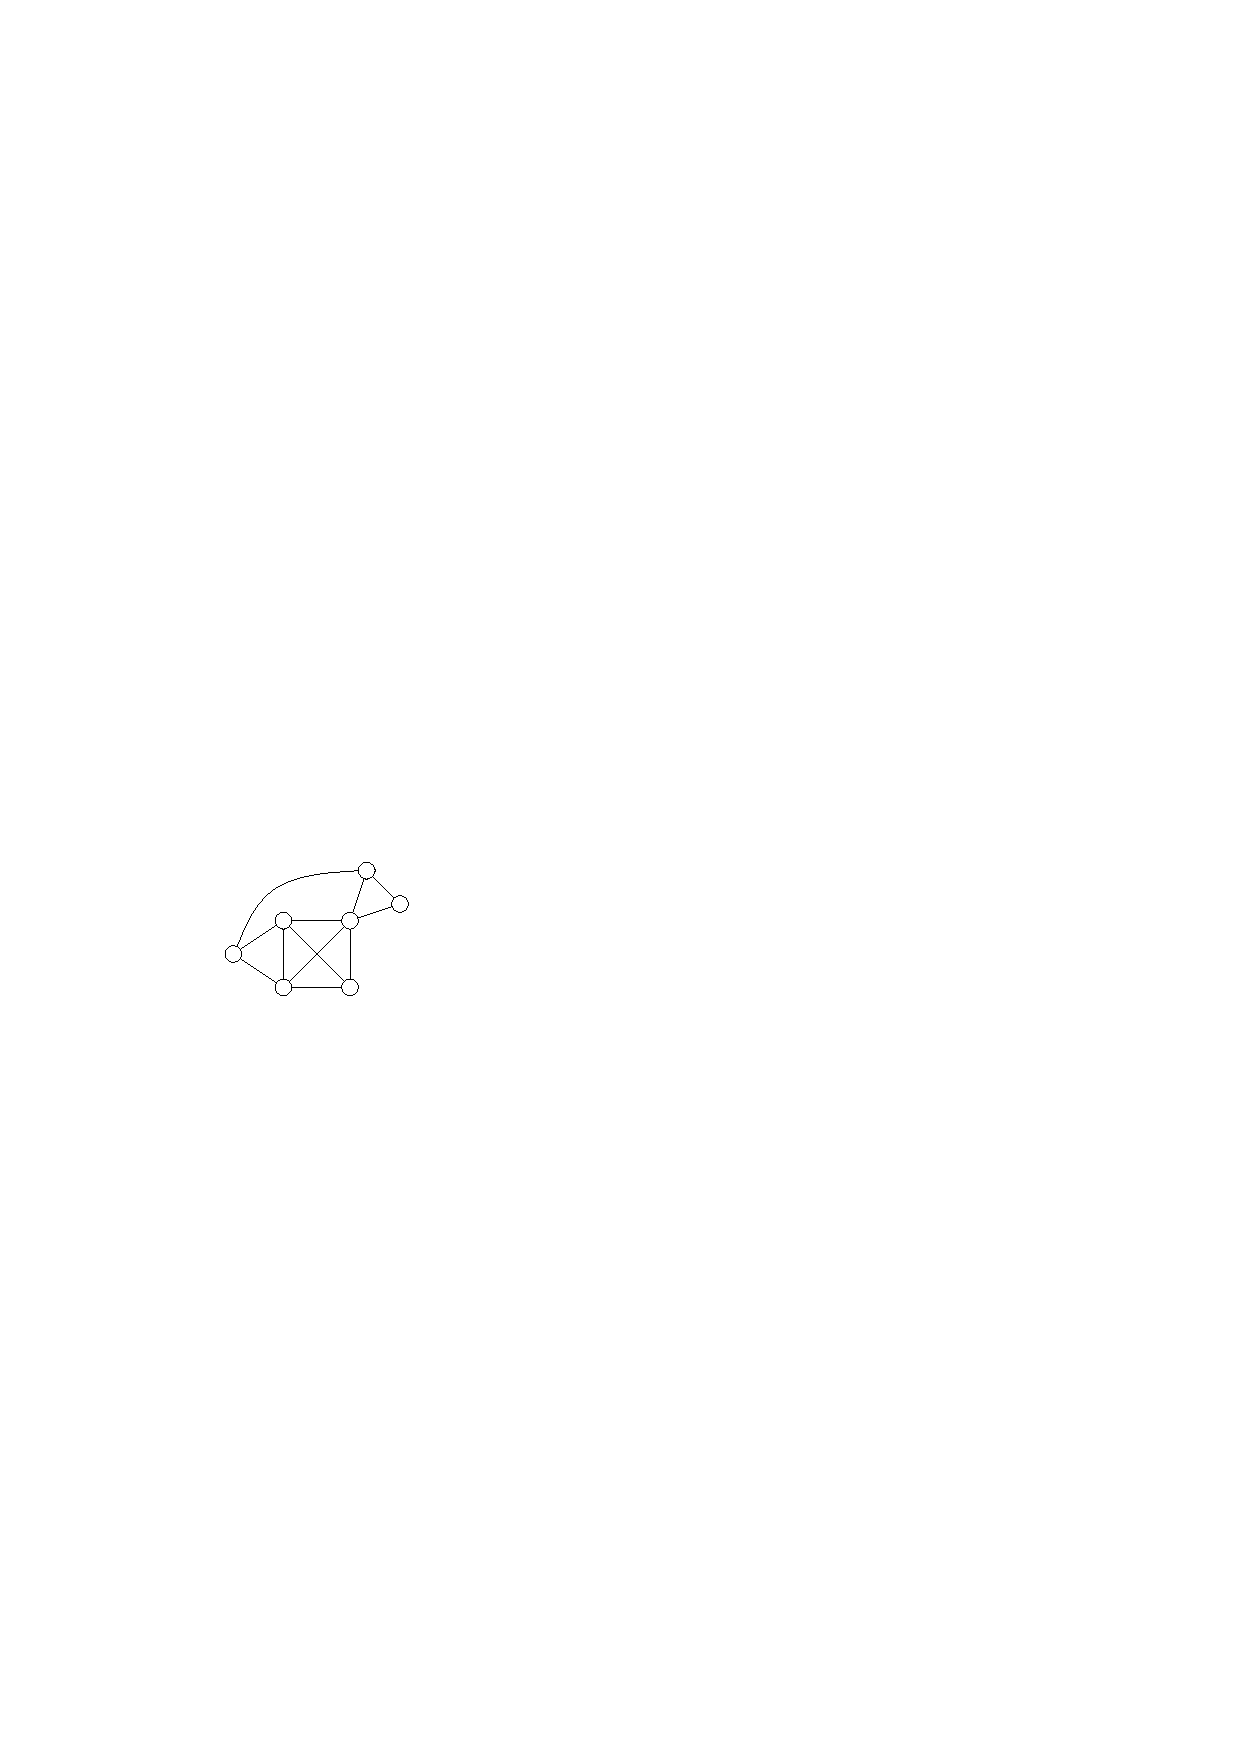
\includegraphics[scale=1.5]{images/tut7-graph}\end{center}
\end{frame}

\section{Mengenprobleme}
\subsection{}

\begin{frame}
\frametitle{EXACT COVER}
\begin{block}{Problem}
\textbf{Gegeben:} Eine Menge $\mathcal{S}$ von Teilmengen einer Menge $X$\\
\textbf{Frage:} Gibt es eine Teilmenge $\mathcal{S}^*$ von $\mathcal{S}$, sodass jedes Element aus $X$ in genau einem der $s \in \mathcal{S}^*$ enthalten ist?
\end{block}
\end{frame}

\begin{frame}
\frametitle{Sudoku}
Sudoku lässt sich als EXACT-COVER Instanz formulieren!\\
Definiere:\\
Sei $V = \{1,2,\ldots,9\}$ die Menge der möglichen Lösungen für ein Kästchen.
Sei $S = \{s_{11}, s_{12},\ldots,s_{19},s_{21},\ldots,s_{99}\}$ die Menge der Sudokukästchen.
Seien weiterhin $r_i = \{s_{i1}, s_{i2}, \ldots s_{i9}\}$ eine Reihe und $R$ die Menge der Reihen.
Analog sei $c_i = \{s_{1i}, s_{2i}, \ldots, s_{9i}\}$ eine Spalte und $C$ die Menge der Spalten.
Seien nun noch $b_k$ die Kästchen, die zum Block $k$ gehören, und $B$ die Menge der Blöcke.
%Hier sollte man alles mal an die Tafel schreiben, sonst ist das zu unübersichtlich ^^
\end{frame}

\begin{frame}
\frametitle{Sudoku}
Betrachte nun die folgende Menge: $U := R \times C \cup R \times V \cup C \times V \cup B \times V$, $U$ ist unsere Menge $X$ (aus der Formulierung des EXACT-COVER-Problems).\\
Definiere: $S_{ijkl} := \{(r_i,c_j),(r_i,v_l),(c_j,v_l),(b_k,v_l)\} \subset U$.\\[8pt]
Wird $S_{ijkl}$ in die Lösung aufgenommen, so kodiert dies, dass im Kästchen $s_{ij}$ im Block $b_k$ der Wert $v_l$ steht.\\
Die Menge $M$ aller $S_{ijkl}$ ist unsere Menge an Teilmengen.\\
Um zu garantieren, dass in einem bestimmten Feld $s_{i'j'}$ eine bestimmte Zahl $v_{l'}$ steht, kann man einfach die $S_{ijkl}$ mit $i = i'$ und $j = j'$ sowie $l \neq l'$ aus $M$ entfernen.
\end{frame}

\begin{frame}
\frametitle{SUBSET-SUM}
\begin{block}{Problem}
\textbf{Gegeben:}
\begin{itemize}
 \item Eine Menge $S$ von Ganzzahlen
 \item Eine Ganzzahl $n$.
\end{itemize}
\textbf{Frage:}
Gibt es eine Teilmenge $S^*$, sodass die Summe der Elemente von $S^*$ gleich $n$ ist?
\end{block}
\end{frame}
%% - PARTITION
\begin{frame}
\frametitle{PARTITION}
\begin{block}{Problem}
\textbf{Gegeben:} Eine Menge von natürlichen Zahlen\\
\textbf{Frage:} Kann man diese Zahlen in zwei Gruppen aufteilen, sodass die Summe der Zahlen in den beiden Gruppen jeweils gleich ist?
\end{block}
\end{frame}

%\begin{frame}
%\frametitle{BIN-PACKING}
%\begin{block}{Problem}
%\textbf{Gegeben:}
%\begin{itemize}
% \item Eine Anzahl $K$ an Behältern der Größe $b \in \mathbb{N}$ und eine Anzahl $n \in \mathbb{N}$ ''Objekte'' mit den Gewichten $a_1, a_2,\ldots,a_n$.
%\end{itemize}
%\textbf{Frage:}
%Können die Objekte so auf die Behälter verteilt werden, dass keiner der Behälter Objekte enthält, deren Gewicht in der Summe $b$ übersteigt?
%\end{block}
%\end{frame}

\section{Mehr Graphenprobleme}
\subsection{}

\begin{frame}
\frametitle{Aufgabe}
Ein Vertex-Cover eines Graphen $G=(V,E)$ ist eine Teilmenge $V'\subseteq V$, so
dass jede Kante aus $E$ zu mindestens einem Knoten aus $V'$ inzident ist.

Das Problem \textsc{VERTEX COVER} besteht nun darin, zu entscheiden, ob es
für einen Graphen $G=(V,E)$ und einen Parameter $k \leq |V|$ ein Vertex-Cover
der Größe höchstens $k$ gibt.

\begin{enumerate}
	\item Finde in folgendem Graphen ein Vertex-Cover minimaler Größe: 
	
		\begin{center}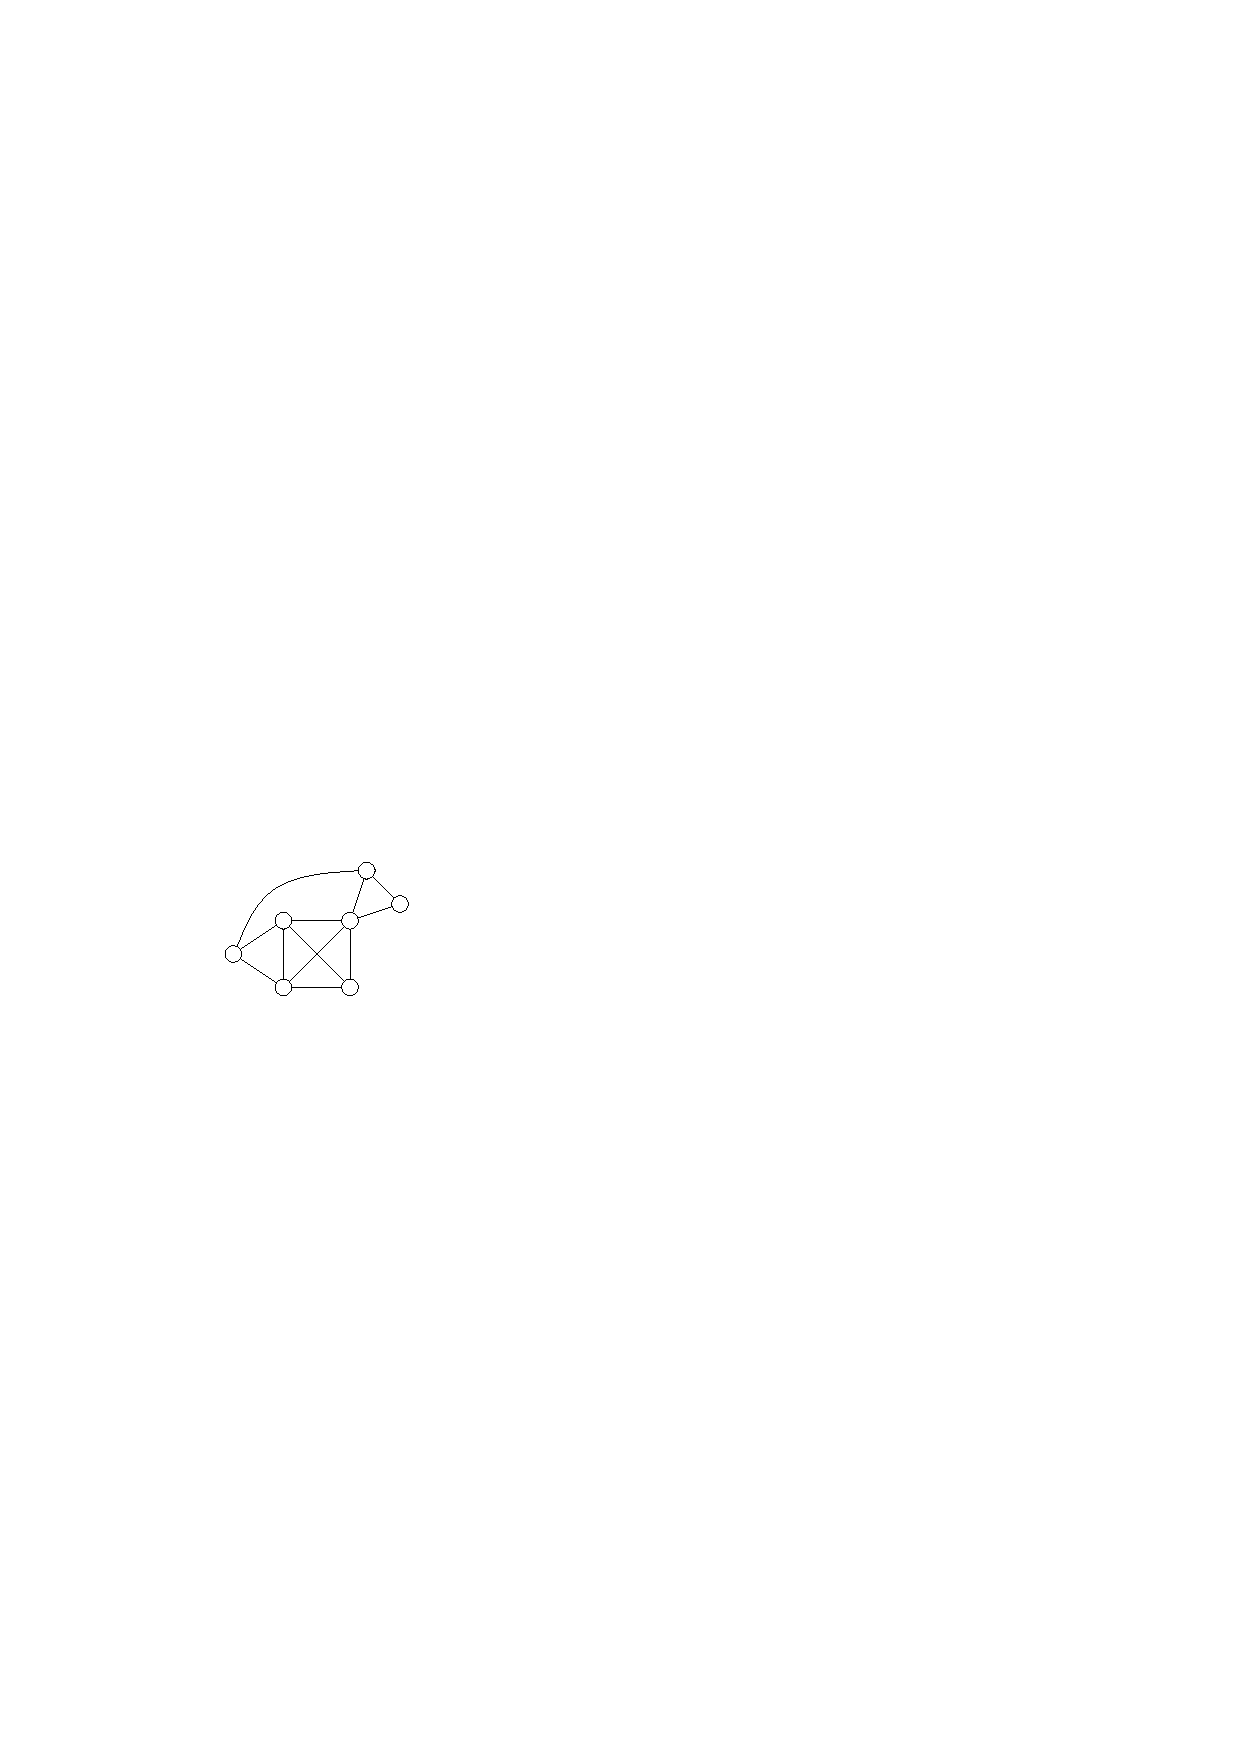
\includegraphics[scale=1.2]{images/tut7-graph}\end{center}
		
	\item Zeige, dass \textsc{VERTEX COVER} $\cal{NP}$-vollständig ist. 
\end{enumerate}
\end{frame}

\begin{frame}
	\frametitle{Lösungsskizze}
	
	\textbf{VERTEX COVER $\in \classNP$:} Für eine gegebene Menge $V'$ kann in Polyzeit überprüft werden, ob sie eine Teilmenge von $V$ ist und alle Kanten von $G$ zu mindestens einem Knoten aus $V'$ inzident sind.
	
	\pause \ducttape{.3cm}
	
	\textbf{VERTEX COVER \classNP{}-schwer:} Reduktion von INDEPENDENT SET:
	
	\begin{itemize}
		\item Gegeben eine Instanz $(G = (V,E), K)$ von INDEPENDENT SET.
		\item Konstruiere daraus eine Instanz $(G' = G, K' = \abs{V} - K)$ von VERTEX COVER (geht offensichtlich in Polyzeit).
		\pause	\item Behauptung: Es gibt ein Independent Set mit Größe $K$ in $G$ \\ $\Leftrightarrow$ Es gibt ein Vertex Cover der Größe $\abs{V} - K$ von $G$.
		\pause \item Beweis: $V' \subseteq V$ ist Independent Set der Größe $K$ \\ $\Leftrightarrow$ Keine zwei Knoten aus $V'$ sind durch eine Kante verbunden \\ $\Leftrightarrow$ Jede Kante ist zu höchstens einem Knoten aus $V'$ inzident \\ $\Leftrightarrow$ Jede Kante ist zu mindestens einem Knoten aus $V \setminus V'$ inzident \\ $\Leftrightarrow$ $V \setminus V'$ ist ein Vertex Cover von $G$ $\qedhere$
	\end{itemize}
\end{frame}

\section{Mehr Mengenprobleme}
\subsection{}

\begin{frame}
 \frametitle{KNAPSACK}
 
 \begin{block}{Problem}
 \textbf{Gegeben:} $(M, w, c, W, C)$
 \begin{itemize}
  \item endliche Menge von Objekten $M$
  \item Gewichtsfunktion $w:M \rightarrow \mathbb{N}_0$
  \item Wertfunktion $c:M \rightarrow \mathbb{N}_0$
  \item Maximalgewicht $W$ und Minimalwert $C$ $\in \N_0$
 \end{itemize}
 \end{block}
 
\textbf{Frage:} Existiert eine Teilmenge $M' \subseteq M$ mit $$\sum_{a\in M'} w(a) \leq W \text{ und } \sum_{a\in  M'} c(a) \geq C\text{  ?}$$

\pause

Was wären das zugehörige Optimalwertproblem und Optimierungsproblem?
\end{frame}

\begin{frame}
 \frametitle{KNAPSACK - Beispiel}
 Gegeben: Instanz $I$ von KNAPSACK mit $M = {i_1, i_2, i_3, i_4}$
  \begin{center}
\begin{tabular}{l|l|l|l|l}
	  &$i_1$ &$i_2$ &$i_3$ 	&$i_4$\\
  \hline
	w &10	 &5	&5	&8\\
  \hline
	c &7	 &10	&5	&8\\	
\end{tabular}
\end{center}
\begin{itemize}
 \item $W$ = 15
 \item $C$ = 18
\end{itemize}
Ist $I$ eine Ja-Instanz?
\end{frame}

\begin{frame}
\frametitle{Lösungsansätze}
\begin{block}{Orakel}
  $M' = \{i_2$, $i_4\}$ ist eine gültige Lösung. $I$ ist somit eine Ja-Instanz.
 \end{block}
\begin{block}{Exponentieller Ansatz}
 Teste alle $2^4 = 16$ mögliche Teilmengen $M' \subseteq M$, ob sie die Bedingung erfüllen. 
\end{block}
\begin{block}{Greedy-Ansatz -- nicht immer optimal}
 Sortiere die Elemente $i \in M$ nach dem Verhältnis $c(i)/w(i)$. 
 Füge so lange Elemente mit dem besten Verhältnis aller $i \not\in M'$ zu $M'$ hinzu, solange $\sum_{i \in M'} w(i) \leq W$ mit dem hinzugefügten Element noch gilt.
 
 Informell: Möglichst wertvolle Dinge einpacken, bis der Rucksack voll ist.
\end{block}
\pause
\begin{block}{}
 Welchen dieser Ansätze verfolgt eine NDTM?
\end{block}

\end{frame}





\begin{frame}
\frametitle{Aufgabe}
Gegeben sei folgende Instanz $I=(M, w, c, W, C)$ von KNAPSACK:

\begin{itemize}
\item $M := \{x_1, \ldots, x_7\}$
\item Gewichtsfunktion $w$ und die Kostenfunktion $c$ sind durch folgende Tabelle gegeben:

\begin{center}
\begin{tabular}{l|l|l|l|l|l|l|l}
	  &$x_1$ &$x_2$ &$x_3$ 	&$x_4$ 	&$x_5$ 	&$x_6$ 	&$x_7$\\ 	
  \hline
	w &6	 &6	&5	&5	&3	&4	&1\\
  \hline
	c &8	 &10	&8	&8	&5	&6	&2\\
\end{tabular}
\end{center}
\item Die obere Schranke für das Gewicht sei $W:=12$
\end{itemize}

Für welche $C$ ist $I$ eine Ja-Instanz?  
\end{frame}

\section{Schluss}
\subsection{Ham}

\begin{frame}
\frametitle{Und viele mehr!}
Es gibt (sehr) viele Probleme, von denen man weiß, dass sie $NP$-vollständig sind. Es gibt ein "`klassisches"' Paper von Richard Karp, in dem 21 Probleme vorgestellt werden, die großteils recht bekannt sind.\\
Wer nicht genug bekommen kann, darf in "`Introduction to the Theory of Computation"' von Michael Sipser schauen, dort gibt es sehr viele.\\[10pt]
Es kann durchaus nützlich sein zu wissen, dass ein Problem $\mathcal{NP}$-vollständig ist; dann kann man aufhören, nach einem effizienten Algorithmus zu suchen.
\end{frame}

\begin{frame}
	\frametitle{Bis zum nächsten Mal!}
	
	\begin{figure}[H]
		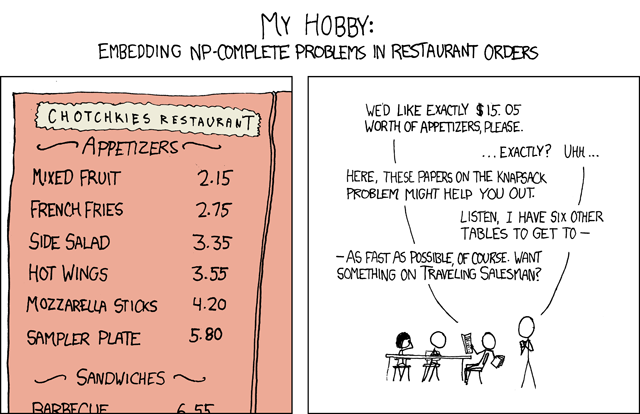
\includegraphics[height=0.8 \textheight]{images/287_np_complete.png}
		
		\textit{\scriptsize{General solutions get you a 50\% tip.}}
	\end{figure}
\end{frame}

\frame{
  \frametitle{Lizenzen}
  \center
  \includegraphics[width=2em]{images/by}
  \includegraphics[width=2em]{images/cc}
  \includegraphics[width=2em]{images/sa}
  \\
  {\tiny

Dieses Werk ist unter einem ``Creative Commons Namensnennung-Weitergabe unter gleichen Bedingungen 3.0 Deutschland``-Lizenzvertrag lizenziert. Um eine Kopie der Lizenz zu erhalten, gehen Sie bitte zu \href{http://creativecommons.org/licenses/by-sa/3.0/de/}{http://creativecommons.org/licenses/by-sa/3.0/de/} oder schreiben Sie an Creative Commons, 171 Second Street, Suite 300, San Francisco, California 94105, USA.\\
  \vspace{1cm}
  Davon ausgenommen sind das Titelbild, welches aus der März-April 2002 Ausgabe von American Scientist erschienen ist und ohne Erlaubnis verwendet wird, sowie das KIT Beamer Theme. Hierfür gelten die Bestimmungen der jeweiligen Urheber.
  \vspace{1cm}
  \\ 
  }
  %Habe hier die Reihenfolge etwas umgestellt, weil die Formatierung bei mir komisch aussah. 
  %Wenn es bei dir anders ist, kannst du es auch wieder zurückändern, dann haben wir unterschiedliche Kompilieroptionen
}

\end{document}
